\subsection{Estimated Speedup Factor}
We computed and estimation of Amdahl's Law on the 3DM benchmark on DUT 2. To compute Amdahl's law we are required to know the paralizable part of the benchmark. Because we do not have the source code for the benchmark this has to be estimated. Each measurements starts with a time period where the system is essential idle, then 3DM executes, which is followed by another period of the DUT being idle. We assume that the period where 3DM is being executed is the paralizable part of the whole measurement, while the periods before and after are serial. Based on this assumption we gathered estimates of the paralizable and serial parts of the measurement. Then we computed estimated speedup and compared it with the actual speedup.

%\begin{figure}[H]
    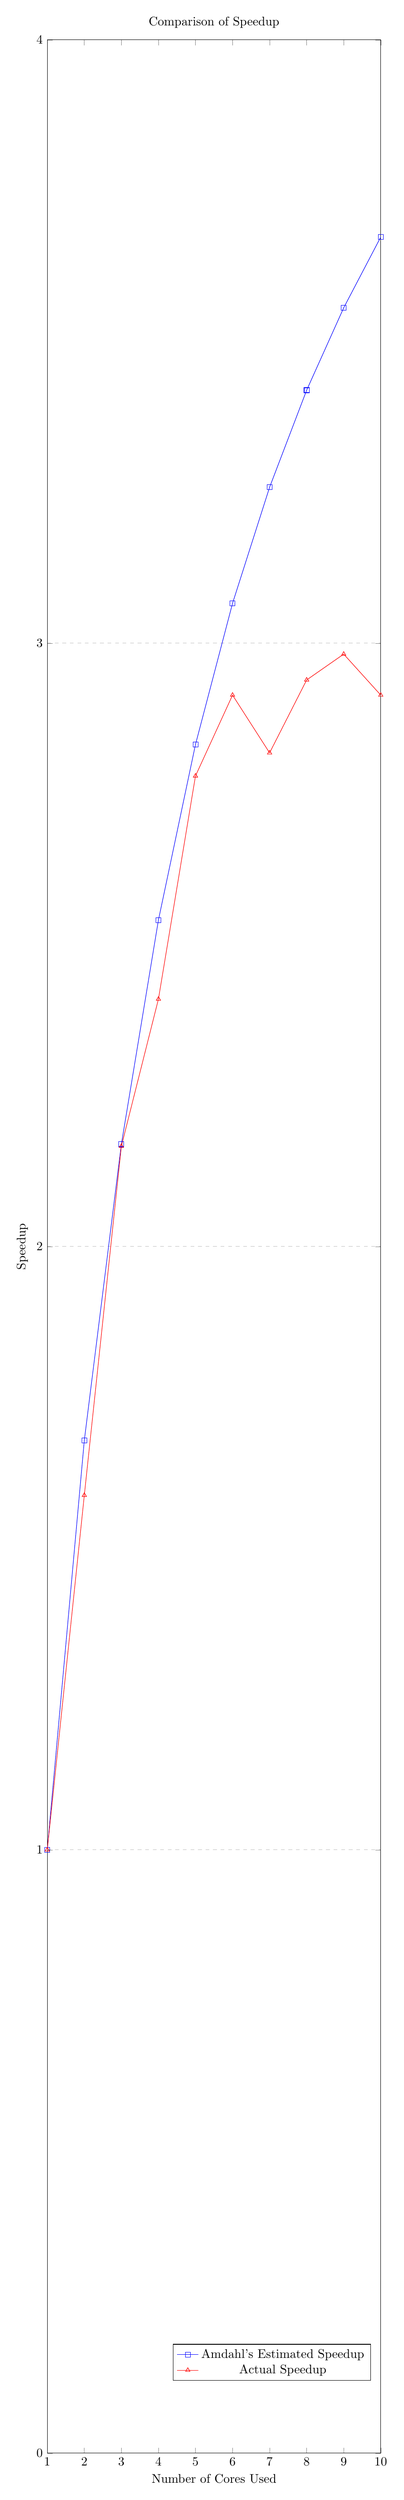
\begin{tikzpicture}
    \begin{axis}[
        title={Comparison of Speedup},
        xlabel={Number of Cores Used},
        ylabel={Speedup},
        xmin=1, xmax=10,
        ymin=0, ymax=4,
        xtick={1,2,3,4,5,6,7,8,9,10},
        ytick={0,1,2,3,4},
        legend pos=south east,
        ymajorgrids=true,
        grid style=dashed,
    ]
    
    \addplot[
        color=blue,
        mark=square,
        ]
        coordinates {
        (1,1)(2,1.6787346222)(3,2.1695941855)(4,2.5411013569)(5,2.8320683114)(6,3.0661245456)(7,3.2584795325)(8,3.4193663866)(9,3.5559232301)(10,3.6732810342)
        };
        \addlegendentry{Amdahl's Estimated Speedup}
    
    \addplot[
        color=red,
        mark=triangle,
        ]
        coordinates {
        (1,1)(2,1.5877659574)(3,2.1663138796)(4,2.4100925147)(5,2.7799767171)(6,2.9139719341)(7,2.8182533438)(8,2.9390769231)(9,2.9818938606)(10,2.9139719341)
        };
        \addlegendentry{Actual Speedup}
    
    \end{axis}
    \end{tikzpicture}
    \caption{A comparison on the estimated speedup from Amdahl's law and the actual Speedup for 3DM on DUT 2}\label{fig:amdahls}
%\end{figure}


On \cref{fig:amdahls} we can see that at after 6 cores Amdahl's estimated speedup factor continuous to increase, while the actual speedup factor stagnates. On this figure the first 6 cores are the P-cores and the last 4 cores are the E-cores. The results show that the E-cores are unable to contribute in speeding up the benchmark. It should be noted that Amdahl's law is intended for processors with identical cores and therefore not the P- and E-core setup. Another factor which may contribute to the stagnation is that the GPU could be the bottleneck. (Perhaps test this by using our GPU).



There is an extension of Amdahl's law to estimate energy consumption by using a fraction for the power the processer uses in idle. We take the average energy consumption in of the whole CPU when idle, and divide 







%\begin{figure}[H]
    \centering
    \begin{tikzpicture}[]
        \pgfplotsset{
            width=0.9\textwidth,
            height=0.12000000000000001\textheight
        }
        \begin{axis}[
            xlabel={Average Energy Consumption (Joules)}, 
            title={The energy consumption of the CPU}, 
            ytick={1},
        yticklabels={
            
            },
            xmin=0,xmax=2000,
            ]
        
        
        \addplot+ [boxplot prepared={
                lower whisker=1489.5706571147173,
                lower quartile=1583.1154519814863,
                median=1615.5316005827935,
                upper quartile=1645.6087846055518,
                upper whisker=1737.4591176664476
                }, color = red
                ] coordinates{(0,1483.827720539599)(0,1480.515622083367)(0,1477.186355372853)(0,1484.2542159930651)(0,1482.5687850286024)(0,1483.6886385780797)(0,1480.4448091317588)(0,1485.3853384265817)(0,1489.3191427731028)(0,1458.8601037522074)(0,1463.0637065063054)(0,1459.2633032605609)(0,1463.5103968722572)(0,1453.1487661688727)(0,1466.0928218042905)(0,1462.0440278870592)(0,1474.5194689908385)(0,1459.453581118759)(0,1457.5866303339164)(0,1455.628237561651)(0,1470.6904548444381)(0,1465.829114695027)(0,1435.7950365323163)(0,1451.3850934121165)(0,1445.9428217597722)(0,1442.063317550344)(0,1450.85856286103)(0,1450.025244877782)(0,1444.8328936770865)(0,1442.6141257907118)(0,1434.7673544518095)(0,1456.5349029807376)(0,1456.5349029807376)(0,1456.5349029807376)(0,1469.107800917624)(0,1455.7667236877767)(0,1446.3544054848612)(0,1440.478635594202)(0,1429.3804508098603)(0,1442.487096133233)(0,1447.3371517815824)(0,1448.3951124219602)(0,1443.5119725972975)(0,1449.5163490103141)(0,1448.3067966005326)(0,1444.8091722080776)(0,1488.3183231268938)(0,1428.9978407533936)(0,1438.5930417864229)(0,1439.4444292808425)(0,1419.3355384521078)(0,1430.0233536758387)(0,1433.6798784909665)(0,1463.3271265226324)(0,1473.3749817250266)(0,1454.68006091368)(0,1461.166059957837)(0,1464.1691792646925)(0,1448.2625544976763)(0,1471.9654808068576)(0,1482.7121745053578)(0,1468.1839213194376)(0,1451.5281583780363)(0,1465.8259684175885)(0,1464.4381879159478)(0,1459.6790065911007)(0,1466.8005289813125)(0,1484.0637126495876)(0,1473.9382777009753)(0,1476.3110273424193)(0,1487.182863469807)(0,1485.3623626131953)(0,1477.8177597132262)(0,1469.9854660438207)(0,1458.7902924145042)(0,1469.2367555649196)(0,1466.3037684311203)(0,1462.5409018030846)(0,1471.0625240925426)(0,1466.1325118899983)(0,1458.7909029714115)(0,1458.4726176585843)(0,1468.8883484124706)(0,1489.1744851861247)(0,1469.2499265102904)(0,1445.2026482875078)(0,1458.109816163985)(0,1457.6681791183883)(0,1447.210046089875)(0,1452.5439302397951)(0,1440.067501240273)(0,1450.621057904693)(0,1448.6112931692753)(0,1438.8810180718888)(0,1453.9687719910191)(0,1443.308717107961)(0,1445.886338736365)(0,1444.2062591436138)(0,1438.9742910237826)(0,1437.3807788196084)(0,1444.3130627858209)(0,1437.5193554744426)(0,1446.2757302195546)(0,1471.6490899927535)(0,1473.0364602217815)(0,1465.8812037103726)(0,1482.1048673399748)(0,1474.5400951339918)(0,1479.0393229368665)(0,1484.9790567800792)(0,1487.9461254357861)(0,1474.0350249535575)(0,1480.1687424911804)(0,1484.3139100818107)(0,1469.8967129422374)(0,1465.9204798921)(0,1460.450840001297)(0,1459.9747522807556)(0,1471.4913887987723)(0,1469.8146428872344)(0,1489.2223694315546)(0,1485.490281176749)(0,1465.3617236871219)(0,1460.420256204019)(0,1487.436311066544)(0,1483.9673066644125)(0,1483.3627965106336)(0,1479.3004350486074)(0,1486.4577228157075)(0,1488.922135610944)(0,1483.1164795925802)(0,1464.9434564910907)(0,1483.122132365524)(0,1479.5559143828937)(0,1483.8150672569302)(0,1482.59893738366)(0,1464.604597534015)(0,1486.7517443309323)(0,1467.346765863508)(0,1473.3181980099016)(0,1484.744285966281)(0,1487.900001883196)(0,1484.2134568699225)(0,1489.1139534455092)(0,1485.5890375229292)(0,1467.947013206326)(0,1480.7963397532792)(0,1466.7648624654041)(0,1478.4261459752838)(0,1475.0392631076127)(0,1469.9205253148295)(0,1467.0255104935788)(0,1471.8492130520733)(0,1477.1480902605667)(0,1463.1183190488334)(0,1465.6677270209457)(0,1469.8791229393983)(0,1458.414271005392)(0,1460.8833782040952)(0,1477.6932897000693)(0,1484.3652169599272)(0,1461.8701133046413)(0,1476.0837910806947)(0,1470.6894084235532)(0,1476.1238727479943)(0,1486.5285697577397)(0,1486.9437870664344)(0,1480.192192757579)(0,1482.354630268667)(0,1485.8874763178158)(0,1488.1373316429483)(0,1475.8172507150293)(0,1471.1667617879066)(0,1473.4804708691138)(0,1463.523181192598)(0,1461.0425510025095)(0,1483.6568318990546)(0,1463.573238317847)(0,1465.8303071048674)(0,1462.6828493352405)(0,1452.727032051925)(0,1463.8366885001133)(0,1459.4660276566972)(0,1463.1992842994848)(0,1462.1255989764634)(0,1474.5952634690248)(0,1470.022111668337)(0,1476.6014254913885)(0,1489.0940952705307)(0,1762.2135609798704)(0,1769.7668627891555)(0,1747.347659874166)};
        
        
        \end{axis}
    \end{tikzpicture}
\caption{CPU measurements by Clamp on DUT 2 for test case(s) MB compiled on oneAPI} \label{fig:2-run-clamp-many-times-exp-clamp-mandelbrot.exe-intel-one-api-workstationtwo-cpu-energy_consumption}
\end{figure}
%\begin{figure}[H]
    \centering
    \begin{tikzpicture}[]
        \pgfplotsset{
            width=0.9\textwidth,
            height=0.24000000000000002\textheight
        }
        \begin{axis}[
            xlabel={Average Runtime (s)}, 
            title={The average duration}, 
            ytick={1, 2, 3, 4, 5, 6, 7},
        yticklabels={
             Plug LIN,  RAPL LIN,  Clamp WIN,  IPG WIN,  LHM WIN,  Plug WIN,  SCAP WIN
            },
            xmin=0,xmax=50,
            ]
        
        
        \addplot+ [boxplot prepared={
                lower whisker=30.361,
                lower quartile=30.388,
                median=30.403,
                upper quartile=30.426,
                upper whisker=30.479
                }, color = red
                ] coordinates{(0,30.644)(0,30.789)(0,30.63)(0,30.624)(0,30.63)(0,30.715)(0,30.661)(0,30.682)(0,30.671)(0,30.507)(0,31.248)(0,30.793)(0,30.501)(0,30.593)(0,30.59)(0,30.519)(0,30.485)(0,30.508)(0,30.667)(0,30.683)(0,30.64)(0,30.534)(0,30.511)(0,30.574)(0,30.779)(0,30.546)(0,30.492)(0,30.674)(0,30.89)(0,30.688)(0,30.618)(0,30.59)(0,30.563)(0,30.492)(0,30.949)(0,30.534)(0,30.671)(0,30.531)(0,30.597)(0,30.732)(0,30.706)(0,30.522)};
        
        \addplot+ [boxplot prepared={
                lower whisker=30.358,
                lower quartile=30.374,
                median=30.379,
                upper quartile=30.394,
                upper whisker=30.424
                }, color = red
                ] coordinates{(1,30.448)(1,30.445)(1,30.44)(1,30.425)(1,30.507)(1,30.592)(1,30.431)(1,30.656)(1,30.577)(1,30.487)(1,30.457)(1,30.658)(1,30.792)(1,30.508)(1,30.544)(1,30.778)(1,31.797)(1,30.618)(1,30.46)(1,30.482)(1,30.456)(1,30.427)(1,30.442)(1,30.657)(1,30.577)(1,30.436)(1,30.658)(1,30.509)(1,30.426)(1,30.667)(1,30.687)(1,30.585)(1,30.537)(1,30.54)(1,30.769)(1,30.651)(1,30.425)(1,30.576)(1,30.434)(1,30.442)(1,31.2)(1,30.427)(1,30.523)(1,30.511)(1,30.641)(1,30.789)(1,30.537)(1,30.436)(1,30.436)(1,30.43)(1,30.434)(1,30.532)(1,30.484)(1,30.476)(1,30.595)(1,30.589)(1,30.469)(1,30.442)(1,30.567)};
        
        \addplot+ [boxplot prepared={
                lower whisker=17.523,
                lower quartile=18.876,
                median=19.372,
                upper quartile=19.9655,
                upper whisker=21.528
                }, color = red
                ] coordinates{(2,22.49)(2,21.684)(2,22.322)(2,21.744)(2,21.792)(2,21.625)(2,21.627)};
        
        \addplot+ [boxplot prepared={
                lower whisker=17.005,
                lower quartile=18.811,
                median=19.458,
                upper quartile=20.122999999999998,
                upper whisker=22.038
                }, color = red
                ] coordinates{(3,16.574)(3,22.275)(3,22.401)(3,22.354)(3,22.206)(3,22.532)(3,22.199)(3,22.288)(3,22.435)(3,22.703)(3,22.343)(3,22.87)(3,22.398)(3,22.4)(3,23.335)(3,23.514)(3,22.099)(3,22.228)(3,22.427)(3,22.677)(3,22.816)(3,22.769)};
        
        \addplot+ [boxplot prepared={
                lower whisker=16.939,
                lower quartile=18.7435,
                median=19.2725,
                upper quartile=19.95075,
                upper whisker=21.729
                }, color = red
                ] coordinates{(4,16.57)(4,22.679)(4,23.252)(4,21.954)(4,21.911)(4,21.835)(4,21.825)(4,21.813)(4,21.785)(4,22.857)(4,22.405)(4,22.285)(4,22.889)(4,22.278)(4,22.311)(4,22.18)(4,22.145)(4,22.102)(4,22.115)(4,25.057)(4,22.001)};
        
        \addplot+ [boxplot prepared={
                lower whisker=17.159,
                lower quartile=18.6985,
                median=19.237,
                upper quartile=19.8965,
                upper whisker=21.684
                }, color = red
                ] coordinates{(5,16.875)(5,22.018)(5,22.902)(5,21.819)(5,23.198)(5,22.574)(5,22.49)(5,22.158)(5,21.798)(5,21.926)(5,21.886)(5,22.984)(5,21.872)(5,22.555)(5,21.752)(5,21.769)(5,21.962)(5,22.287)(5,21.698)};
        
        \addplot+ [boxplot prepared={
                lower whisker=16.819,
                lower quartile=18.78775,
                median=19.342,
                upper quartile=20.110500000000002,
                upper whisker=21.879
                }, color = red
                ] coordinates{(6,22.192)(6,22.37)(6,22.368)(6,22.722)(6,22.959)(6,22.479)(6,22.729)(6,24.736)(6,22.898)};
        
        
        \end{axis}
    \end{tikzpicture}
\caption{Runtime measurements on DUT 1 for test case(s) FR compiled on oneAPI} \label{fig:2-same-one-api-compiler-different-measuring-instruments-post-update-and-watt-clamp-ipg-lhm-plug-rapl-rapl-scaphandre-fannkuch-redux.exe-intel-one-api-workstationone-runtime-duration}
\end{figure}

\begin{figure}[H]
    \centering
    \begin{tikzpicture}[]
        \pgfplotsset{
            width=0.9\textwidth,
            height=0.12000000000000001\textheight
        }
        \begin{axis}[
            xlabel={Average Energy Consumption (Joules)}, 
            title={The energy consumption of the CPU}, 
            ytick={1},
        yticklabels={
            
            },
            xmin=0,xmax=2000,
            ]
        
        
        \addplot+ [boxplot prepared={
                lower whisker=1489.5706571147173,
                lower quartile=1583.1154519814863,
                median=1615.5316005827935,
                upper quartile=1645.6087846055518,
                upper whisker=1737.4591176664476
                }, color = red
                ] coordinates{(0,1483.827720539599)(0,1480.515622083367)(0,1477.186355372853)(0,1484.2542159930651)(0,1482.5687850286024)(0,1483.6886385780797)(0,1480.4448091317588)(0,1485.3853384265817)(0,1489.3191427731028)(0,1458.8601037522074)(0,1463.0637065063054)(0,1459.2633032605609)(0,1463.5103968722572)(0,1453.1487661688727)(0,1466.0928218042905)(0,1462.0440278870592)(0,1474.5194689908385)(0,1459.453581118759)(0,1457.5866303339164)(0,1455.628237561651)(0,1470.6904548444381)(0,1465.829114695027)(0,1435.7950365323163)(0,1451.3850934121165)(0,1445.9428217597722)(0,1442.063317550344)(0,1450.85856286103)(0,1450.025244877782)(0,1444.8328936770865)(0,1442.6141257907118)(0,1434.7673544518095)(0,1456.5349029807376)(0,1456.5349029807376)(0,1456.5349029807376)(0,1469.107800917624)(0,1455.7667236877767)(0,1446.3544054848612)(0,1440.478635594202)(0,1429.3804508098603)(0,1442.487096133233)(0,1447.3371517815824)(0,1448.3951124219602)(0,1443.5119725972975)(0,1449.5163490103141)(0,1448.3067966005326)(0,1444.8091722080776)(0,1488.3183231268938)(0,1428.9978407533936)(0,1438.5930417864229)(0,1439.4444292808425)(0,1419.3355384521078)(0,1430.0233536758387)(0,1433.6798784909665)(0,1463.3271265226324)(0,1473.3749817250266)(0,1454.68006091368)(0,1461.166059957837)(0,1464.1691792646925)(0,1448.2625544976763)(0,1471.9654808068576)(0,1482.7121745053578)(0,1468.1839213194376)(0,1451.5281583780363)(0,1465.8259684175885)(0,1464.4381879159478)(0,1459.6790065911007)(0,1466.8005289813125)(0,1484.0637126495876)(0,1473.9382777009753)(0,1476.3110273424193)(0,1487.182863469807)(0,1485.3623626131953)(0,1477.8177597132262)(0,1469.9854660438207)(0,1458.7902924145042)(0,1469.2367555649196)(0,1466.3037684311203)(0,1462.5409018030846)(0,1471.0625240925426)(0,1466.1325118899983)(0,1458.7909029714115)(0,1458.4726176585843)(0,1468.8883484124706)(0,1489.1744851861247)(0,1469.2499265102904)(0,1445.2026482875078)(0,1458.109816163985)(0,1457.6681791183883)(0,1447.210046089875)(0,1452.5439302397951)(0,1440.067501240273)(0,1450.621057904693)(0,1448.6112931692753)(0,1438.8810180718888)(0,1453.9687719910191)(0,1443.308717107961)(0,1445.886338736365)(0,1444.2062591436138)(0,1438.9742910237826)(0,1437.3807788196084)(0,1444.3130627858209)(0,1437.5193554744426)(0,1446.2757302195546)(0,1471.6490899927535)(0,1473.0364602217815)(0,1465.8812037103726)(0,1482.1048673399748)(0,1474.5400951339918)(0,1479.0393229368665)(0,1484.9790567800792)(0,1487.9461254357861)(0,1474.0350249535575)(0,1480.1687424911804)(0,1484.3139100818107)(0,1469.8967129422374)(0,1465.9204798921)(0,1460.450840001297)(0,1459.9747522807556)(0,1471.4913887987723)(0,1469.8146428872344)(0,1489.2223694315546)(0,1485.490281176749)(0,1465.3617236871219)(0,1460.420256204019)(0,1487.436311066544)(0,1483.9673066644125)(0,1483.3627965106336)(0,1479.3004350486074)(0,1486.4577228157075)(0,1488.922135610944)(0,1483.1164795925802)(0,1464.9434564910907)(0,1483.122132365524)(0,1479.5559143828937)(0,1483.8150672569302)(0,1482.59893738366)(0,1464.604597534015)(0,1486.7517443309323)(0,1467.346765863508)(0,1473.3181980099016)(0,1484.744285966281)(0,1487.900001883196)(0,1484.2134568699225)(0,1489.1139534455092)(0,1485.5890375229292)(0,1467.947013206326)(0,1480.7963397532792)(0,1466.7648624654041)(0,1478.4261459752838)(0,1475.0392631076127)(0,1469.9205253148295)(0,1467.0255104935788)(0,1471.8492130520733)(0,1477.1480902605667)(0,1463.1183190488334)(0,1465.6677270209457)(0,1469.8791229393983)(0,1458.414271005392)(0,1460.8833782040952)(0,1477.6932897000693)(0,1484.3652169599272)(0,1461.8701133046413)(0,1476.0837910806947)(0,1470.6894084235532)(0,1476.1238727479943)(0,1486.5285697577397)(0,1486.9437870664344)(0,1480.192192757579)(0,1482.354630268667)(0,1485.8874763178158)(0,1488.1373316429483)(0,1475.8172507150293)(0,1471.1667617879066)(0,1473.4804708691138)(0,1463.523181192598)(0,1461.0425510025095)(0,1483.6568318990546)(0,1463.573238317847)(0,1465.8303071048674)(0,1462.6828493352405)(0,1452.727032051925)(0,1463.8366885001133)(0,1459.4660276566972)(0,1463.1992842994848)(0,1462.1255989764634)(0,1474.5952634690248)(0,1470.022111668337)(0,1476.6014254913885)(0,1489.0940952705307)(0,1762.2135609798704)(0,1769.7668627891555)(0,1747.347659874166)};
        
        
        \end{axis}
    \end{tikzpicture}
\caption{CPU measurements by Clamp on DUT 2 for test case(s) MB compiled on oneAPI} \label{fig:2-run-clamp-many-times-exp-clamp-mandelbrot.exe-intel-one-api-workstationtwo-cpu-energy_consumption}
\end{figure}
\begin{figure}[H]
    \centering
    \begin{tikzpicture}[]
        \pgfplotsset{
            width=0.9\textwidth,
            height=0.24000000000000002\textheight
        }
        \begin{axis}[
            xlabel={Average Runtime (s)}, 
            title={The average duration}, 
            ytick={1, 2, 3, 4, 5, 6, 7},
        yticklabels={
             Plug LIN,  RAPL LIN,  Clamp WIN,  IPG WIN,  LHM WIN,  Plug WIN,  SCAP WIN
            },
            xmin=0,xmax=50,
            ]
        
        
        \addplot+ [boxplot prepared={
                lower whisker=30.361,
                lower quartile=30.388,
                median=30.403,
                upper quartile=30.426,
                upper whisker=30.479
                }, color = red
                ] coordinates{(0,30.644)(0,30.789)(0,30.63)(0,30.624)(0,30.63)(0,30.715)(0,30.661)(0,30.682)(0,30.671)(0,30.507)(0,31.248)(0,30.793)(0,30.501)(0,30.593)(0,30.59)(0,30.519)(0,30.485)(0,30.508)(0,30.667)(0,30.683)(0,30.64)(0,30.534)(0,30.511)(0,30.574)(0,30.779)(0,30.546)(0,30.492)(0,30.674)(0,30.89)(0,30.688)(0,30.618)(0,30.59)(0,30.563)(0,30.492)(0,30.949)(0,30.534)(0,30.671)(0,30.531)(0,30.597)(0,30.732)(0,30.706)(0,30.522)};
        
        \addplot+ [boxplot prepared={
                lower whisker=30.358,
                lower quartile=30.374,
                median=30.379,
                upper quartile=30.394,
                upper whisker=30.424
                }, color = red
                ] coordinates{(1,30.448)(1,30.445)(1,30.44)(1,30.425)(1,30.507)(1,30.592)(1,30.431)(1,30.656)(1,30.577)(1,30.487)(1,30.457)(1,30.658)(1,30.792)(1,30.508)(1,30.544)(1,30.778)(1,31.797)(1,30.618)(1,30.46)(1,30.482)(1,30.456)(1,30.427)(1,30.442)(1,30.657)(1,30.577)(1,30.436)(1,30.658)(1,30.509)(1,30.426)(1,30.667)(1,30.687)(1,30.585)(1,30.537)(1,30.54)(1,30.769)(1,30.651)(1,30.425)(1,30.576)(1,30.434)(1,30.442)(1,31.2)(1,30.427)(1,30.523)(1,30.511)(1,30.641)(1,30.789)(1,30.537)(1,30.436)(1,30.436)(1,30.43)(1,30.434)(1,30.532)(1,30.484)(1,30.476)(1,30.595)(1,30.589)(1,30.469)(1,30.442)(1,30.567)};
        
        \addplot+ [boxplot prepared={
                lower whisker=17.523,
                lower quartile=18.876,
                median=19.372,
                upper quartile=19.9655,
                upper whisker=21.528
                }, color = red
                ] coordinates{(2,22.49)(2,21.684)(2,22.322)(2,21.744)(2,21.792)(2,21.625)(2,21.627)};
        
        \addplot+ [boxplot prepared={
                lower whisker=17.005,
                lower quartile=18.811,
                median=19.458,
                upper quartile=20.122999999999998,
                upper whisker=22.038
                }, color = red
                ] coordinates{(3,16.574)(3,22.275)(3,22.401)(3,22.354)(3,22.206)(3,22.532)(3,22.199)(3,22.288)(3,22.435)(3,22.703)(3,22.343)(3,22.87)(3,22.398)(3,22.4)(3,23.335)(3,23.514)(3,22.099)(3,22.228)(3,22.427)(3,22.677)(3,22.816)(3,22.769)};
        
        \addplot+ [boxplot prepared={
                lower whisker=16.939,
                lower quartile=18.7435,
                median=19.2725,
                upper quartile=19.95075,
                upper whisker=21.729
                }, color = red
                ] coordinates{(4,16.57)(4,22.679)(4,23.252)(4,21.954)(4,21.911)(4,21.835)(4,21.825)(4,21.813)(4,21.785)(4,22.857)(4,22.405)(4,22.285)(4,22.889)(4,22.278)(4,22.311)(4,22.18)(4,22.145)(4,22.102)(4,22.115)(4,25.057)(4,22.001)};
        
        \addplot+ [boxplot prepared={
                lower whisker=17.159,
                lower quartile=18.6985,
                median=19.237,
                upper quartile=19.8965,
                upper whisker=21.684
                }, color = red
                ] coordinates{(5,16.875)(5,22.018)(5,22.902)(5,21.819)(5,23.198)(5,22.574)(5,22.49)(5,22.158)(5,21.798)(5,21.926)(5,21.886)(5,22.984)(5,21.872)(5,22.555)(5,21.752)(5,21.769)(5,21.962)(5,22.287)(5,21.698)};
        
        \addplot+ [boxplot prepared={
                lower whisker=16.819,
                lower quartile=18.78775,
                median=19.342,
                upper quartile=20.110500000000002,
                upper whisker=21.879
                }, color = red
                ] coordinates{(6,22.192)(6,22.37)(6,22.368)(6,22.722)(6,22.959)(6,22.479)(6,22.729)(6,24.736)(6,22.898)};
        
        
        \end{axis}
    \end{tikzpicture}
\caption{Runtime measurements on DUT 1 for test case(s) FR compiled on oneAPI} \label{fig:2-same-one-api-compiler-different-measuring-instruments-post-update-and-watt-clamp-ipg-lhm-plug-rapl-rapl-scaphandre-fannkuch-redux.exe-intel-one-api-workstationone-runtime-duration}
\end{figure}
\begin{figure}[H]
    \centering
    \begin{tikzpicture}[]
        \pgfplotsset{
            width=0.9\textwidth,
            height=0.28\textheight
        }
        \begin{axis}[
            xlabel={Average DEC (Joules)}, 
            ylabel={Number of Cores},
            title={The DEC of the CPU}, 
            ytick={1, 2, 3, 4, 5, 6, 7, 8, 9},
        yticklabels={
                8,7,6,5,4,3,2,1
        %      4, 3, 2, 1, 5, 0, 8, 7, 6, 9,  4, 3, 2, 1, 5, 0, 8, 7, 6,  4, 3, 2, 1, 5, 0, 8, 7,  4, 3, 2, 1, 5, 0, 8,  4, 3, 2, 1, 5, 0,  4, 3, 2, 1, 5,  4, 3, 2, 1,  4, 3, 2,  4, 3
            },
            xmin=0,xmax=8000,
            ]
        
        
        \addplot+ [boxplot prepared={
                lower whisker=2550.9239986733783,
                lower quartile=2758.6690893693917,
                median=2857.039605504193,
                upper quartile=3031.204295476026,
                upper whisker=3424.0203866976954
                }, color = red
                ] coordinates{(0,3482.0465773339693)};
        
        \addplot+ [boxplot prepared={
                lower whisker=2558.8650387164184,
                lower quartile=2762.7255476887685,
                median=2855.713350935676,
                upper quartile=3045.3451708394396,
                upper whisker=3454.155219761194
                }, color = red
                ] coordinates{(1,3486.4640357170842)};
        
        \addplot+ [boxplot prepared={
                lower whisker=2570.2732239917177,
                lower quartile=2777.1988876087926,
                median=2884.2866151069957,
                upper quartile=3068.1117873283933,
                upper whisker=3454.780082734922
                }, color = red
                ] coordinates{};
        
        \addplot+ [boxplot prepared={
                lower whisker=2602.7958502421834,
                lower quartile=2792.1049336085575,
                median=2888.9162169260862,
                upper quartile=3053.269761232298,
                upper whisker=3389.244331830094
                }, color = red
                ] coordinates{(3,3451.310775686924)(3,3458.840287066336)(3,3504.7905888736705)(3,3483.9311167776605)};
        
        \addplot+ [boxplot prepared={
                lower whisker=2611.1475430861483,
                lower quartile=2820.2788391131394,
                median=2919.395705131882,
                upper quartile=3100.2439880050365,
                upper whisker=3514.7805915573454
                }, color = red
                ] coordinates{(4,3553.3059338611256)};
        
        \addplot+ [boxplot prepared={
                lower whisker=2582.79506257707,
                lower quartile=2805.2295082892288,
                median=2878.891589696851,
                upper quartile=3065.7726962683714,
                upper whisker=3446.877246021614
                }, color = red
                ] coordinates{(5,3520.9853594875676)(5,3486.811717530646)(5,3463.1842972780987)(5,3479.8908294462854)};
        
        \addplot+ [boxplot prepared={
                lower whisker=2574.063753410154,
                lower quartile=2802.763223923163,
                median=2889.4579163141257,
                upper quartile=3071.729862987921,
                upper whisker=3465.599989910425
                }, color = red
                ] coordinates{(6,3551.2723772195336)(6,3494.5064337314247)(6,3480.416707826837)};
        
        \addplot+ [boxplot prepared={
                lower whisker=2591.6156479589,
                lower quartile=2765.5739923110095,
                median=2864.6154389163394,
                upper quartile=3081.8995257679594,
                upper whisker=3540.8256345513973
                }, color = red
                ] coordinates{};
        
        \addplot+ [boxplot prepared={
                lower whisker=2523.581895919968,
                lower quartile=2743.083521651061,
                median=2805.267152358031,
                upper quartile=3057.2664553554314,
                upper whisker=3495.1741632132553
                }, color = red
                ] coordinates{(8,3555.0886503048287)(8,3573.10817891006)};
        
        
        \end{axis}
    \end{tikzpicture}
\caption{CPU measurements by IPG on DUT 2 for test case(s) PCM} \label{fig:3-same-mi-different-application-post-config-update-ipg-pc-mark-10.exe-unkown-workstationtwo-cpu-dec}
\end{figure}



%We can see that after 6 cores the Speedup Factor stagnates and actually slight decreases. This like because the last 4 cores are the E-cores. The decrease could be because the through put of the E cores are lower, which means the P-cores has to wait for them to finish their job.


%\begin{figure}[H]
    \centering
    \begin{tikzpicture}[]
        \pgfplotsset{
            width=0.9\textwidth,
            height=0.12000000000000001\textheight
        }
        \begin{axis}[
            xlabel={Average Energy Consumption (Joules)}, 
            title={The energy consumption of the CPU}, 
            ytick={1},
        yticklabels={
            
            },
            xmin=0,xmax=2000,
            ]
        
        
        \addplot+ [boxplot prepared={
                lower whisker=1489.5706571147173,
                lower quartile=1583.1154519814863,
                median=1615.5316005827935,
                upper quartile=1645.6087846055518,
                upper whisker=1737.4591176664476
                }, color = red
                ] coordinates{(0,1483.827720539599)(0,1480.515622083367)(0,1477.186355372853)(0,1484.2542159930651)(0,1482.5687850286024)(0,1483.6886385780797)(0,1480.4448091317588)(0,1485.3853384265817)(0,1489.3191427731028)(0,1458.8601037522074)(0,1463.0637065063054)(0,1459.2633032605609)(0,1463.5103968722572)(0,1453.1487661688727)(0,1466.0928218042905)(0,1462.0440278870592)(0,1474.5194689908385)(0,1459.453581118759)(0,1457.5866303339164)(0,1455.628237561651)(0,1470.6904548444381)(0,1465.829114695027)(0,1435.7950365323163)(0,1451.3850934121165)(0,1445.9428217597722)(0,1442.063317550344)(0,1450.85856286103)(0,1450.025244877782)(0,1444.8328936770865)(0,1442.6141257907118)(0,1434.7673544518095)(0,1456.5349029807376)(0,1456.5349029807376)(0,1456.5349029807376)(0,1469.107800917624)(0,1455.7667236877767)(0,1446.3544054848612)(0,1440.478635594202)(0,1429.3804508098603)(0,1442.487096133233)(0,1447.3371517815824)(0,1448.3951124219602)(0,1443.5119725972975)(0,1449.5163490103141)(0,1448.3067966005326)(0,1444.8091722080776)(0,1488.3183231268938)(0,1428.9978407533936)(0,1438.5930417864229)(0,1439.4444292808425)(0,1419.3355384521078)(0,1430.0233536758387)(0,1433.6798784909665)(0,1463.3271265226324)(0,1473.3749817250266)(0,1454.68006091368)(0,1461.166059957837)(0,1464.1691792646925)(0,1448.2625544976763)(0,1471.9654808068576)(0,1482.7121745053578)(0,1468.1839213194376)(0,1451.5281583780363)(0,1465.8259684175885)(0,1464.4381879159478)(0,1459.6790065911007)(0,1466.8005289813125)(0,1484.0637126495876)(0,1473.9382777009753)(0,1476.3110273424193)(0,1487.182863469807)(0,1485.3623626131953)(0,1477.8177597132262)(0,1469.9854660438207)(0,1458.7902924145042)(0,1469.2367555649196)(0,1466.3037684311203)(0,1462.5409018030846)(0,1471.0625240925426)(0,1466.1325118899983)(0,1458.7909029714115)(0,1458.4726176585843)(0,1468.8883484124706)(0,1489.1744851861247)(0,1469.2499265102904)(0,1445.2026482875078)(0,1458.109816163985)(0,1457.6681791183883)(0,1447.210046089875)(0,1452.5439302397951)(0,1440.067501240273)(0,1450.621057904693)(0,1448.6112931692753)(0,1438.8810180718888)(0,1453.9687719910191)(0,1443.308717107961)(0,1445.886338736365)(0,1444.2062591436138)(0,1438.9742910237826)(0,1437.3807788196084)(0,1444.3130627858209)(0,1437.5193554744426)(0,1446.2757302195546)(0,1471.6490899927535)(0,1473.0364602217815)(0,1465.8812037103726)(0,1482.1048673399748)(0,1474.5400951339918)(0,1479.0393229368665)(0,1484.9790567800792)(0,1487.9461254357861)(0,1474.0350249535575)(0,1480.1687424911804)(0,1484.3139100818107)(0,1469.8967129422374)(0,1465.9204798921)(0,1460.450840001297)(0,1459.9747522807556)(0,1471.4913887987723)(0,1469.8146428872344)(0,1489.2223694315546)(0,1485.490281176749)(0,1465.3617236871219)(0,1460.420256204019)(0,1487.436311066544)(0,1483.9673066644125)(0,1483.3627965106336)(0,1479.3004350486074)(0,1486.4577228157075)(0,1488.922135610944)(0,1483.1164795925802)(0,1464.9434564910907)(0,1483.122132365524)(0,1479.5559143828937)(0,1483.8150672569302)(0,1482.59893738366)(0,1464.604597534015)(0,1486.7517443309323)(0,1467.346765863508)(0,1473.3181980099016)(0,1484.744285966281)(0,1487.900001883196)(0,1484.2134568699225)(0,1489.1139534455092)(0,1485.5890375229292)(0,1467.947013206326)(0,1480.7963397532792)(0,1466.7648624654041)(0,1478.4261459752838)(0,1475.0392631076127)(0,1469.9205253148295)(0,1467.0255104935788)(0,1471.8492130520733)(0,1477.1480902605667)(0,1463.1183190488334)(0,1465.6677270209457)(0,1469.8791229393983)(0,1458.414271005392)(0,1460.8833782040952)(0,1477.6932897000693)(0,1484.3652169599272)(0,1461.8701133046413)(0,1476.0837910806947)(0,1470.6894084235532)(0,1476.1238727479943)(0,1486.5285697577397)(0,1486.9437870664344)(0,1480.192192757579)(0,1482.354630268667)(0,1485.8874763178158)(0,1488.1373316429483)(0,1475.8172507150293)(0,1471.1667617879066)(0,1473.4804708691138)(0,1463.523181192598)(0,1461.0425510025095)(0,1483.6568318990546)(0,1463.573238317847)(0,1465.8303071048674)(0,1462.6828493352405)(0,1452.727032051925)(0,1463.8366885001133)(0,1459.4660276566972)(0,1463.1992842994848)(0,1462.1255989764634)(0,1474.5952634690248)(0,1470.022111668337)(0,1476.6014254913885)(0,1489.0940952705307)(0,1762.2135609798704)(0,1769.7668627891555)(0,1747.347659874166)};
        
        
        \end{axis}
    \end{tikzpicture}
\caption{CPU measurements by Clamp on DUT 2 for test case(s) MB compiled on oneAPI} \label{fig:2-run-clamp-many-times-exp-clamp-mandelbrot.exe-intel-one-api-workstationtwo-cpu-energy_consumption}
\end{figure}

%C:\Github\BDEnergy\article\tables\results\same-mi-different-application-post-config-update\ipg\3d-mark\workstationtwo\unkown\CPU_energy_consumption.tex

%%%%%%% NEW CALCULATIONS BASED ON AVERAGE %%%%%%%%%%%%%%%%%%
Amdahls law
S(n) = 1/ ((1-p)+p/n)


Parallel start on 1 core = 15 sec
Parallel end on 1 core = 130,86 sec
Benchmark end on1 core: 143.28 sec

Parallel time : 130,86 - 15 = 115,86

Fraction of parallel portion
p = 115,86/ 143,28 = 0,8086264657


AMDAHLS LAW ESTIMATES
S(n) 1/ ((1-0,8086264657)+ (0,8086264657 / 2)) = 1,6787346222
S(n) 1/ ((1-0,8086264657)+ (0,8086264657 / 3)) = 2,1695941855
S(n) 1/ ((1-0,8086264657)+ (0,8086264657 / 4)) = 2,5411013569
S(n) 1/ ((1-0,8086264657)+ (0,8086264657 / 5)) = 2,8320683114
S(n) 1/ ((1-0,8086264657)+ (0,8086264657 / 6)) = 3,0661245456
S(n) 1/ ((1-0,8086264657)+ (0,8086264657 / 7)) = 3,2584795325
S(n) 1/ ((1-0,8086264657)+ (0,8086264657 / 8)) = 3,4193663866
S(n) 1/ ((1-0,8086264657)+ (0,8086264657 / 9)) = 3,5559232301
S(n) 1/ ((1-0,8086264657)+ (0,8086264657 / 10)) = 3,6732810342

End times for 2 cores = 90.24
End times for 3 cores = 66.14
End times for 4 cores = 59.45
End times for 5 cores = 51.54
End times for 6 cores = 49.17
End times for 7 cores = 50.84
End times for 8 cores = 48.75
End times for 9 cores = 48.05
End times for 10 cores = 49.17

Actual Speedup
AS for 2 cores = 143,28 / 90,24 = 1,5877659574
AS for 3 cores = 143,28 / 66,14 = 2,1663138796
AS for 4 cores = 143,28 / 59,45 = 2,4100925147
AS for 5 cores = 143,28 / 51,54 = 2,7799767171
AS for 6 cores = 143,28 / 49,17 = 2,9139719341
AS for 7 cores = 143,28 / 50,84 = 2,8182533438
AS for 8 cores = 143,28 / 48,75 = 2,9390769231
AS for 9 cores = 143,28 / 48,05 = 2,9818938606 
AS for 10 cores = 143,28 / 49,17 = 2,9139719341

36,9 j average idle on DUT 2
In watts = 5.5206430099 W

433.51 j average full load FR on DUT 2.
run time 28.6845
In watts 20.2 W

fraction of power consumption of processer in idle k
k = 5,5206430099 / 20,2 = 0,273

Extension formulas

W = (1 + (n-1)k(1-p)) / ((1 - p) + p/n)
W = (1 + (2-1)0,273(1-0,8086264657)) / ((1 - 0,8086264657) + 0,8086264657/2) = 1,7664400703
W = (1 + (3-1)0,273(1-0,8086264657)) / ((1 - 0,8086264657) + 0,8086264657/3) = 2,3962949728
W = (1 + (4-1)0,273(1-0,8086264657)) / ((1 - 0,8086264657) + 0,8086264657/4) = 2,9393806865
W = (1 + (5-1)0,273(1-0,8086264657)) / ((1 - 0,8086264657) + 0,8086264657/5) = 3,4239136624
W = (1 + (6-1)0,273(1-0,8086264657)) / ((1 - 0,8086264657) + 0,8086264657/6) = 3,8670725446
W = (1 + (7-1)0,273(1-0,8086264657)) / ((1 - 0,8086264657) + 0,8086264657/7) = 4,2799146201
W = (1 + (8-1)0,273(1-0,8086264657)) / ((1 - 0,8086264657) + 0,8086264657/8) = 4,6698793631
W = (1 + (9-1)0,273(1-0,8086264657)) / ((1 - 0,8086264657) + 0,8086264657/9) = 5,0421561883
W = (1 + (10-1)0,273(1-0,8086264657)) / ((1 - 0,8086264657) + 0,8086264657/10) = 5,4004753118

Actual energy consumption in Joules to Watt for DUT 2 on 3DM
1 core 1458.66
Run time = 164,63
8,8602320355 W
Idle = 909,1406800494 j

Idle W = 5,5223269152 W

337 j over 61.025 s
1462 1 core for 164
5,5223269152 W 

2 core 1145.49
Run time = 107,221
10,6834482051 W
Idle W = (Total - DEC) / Run time
Idle = (1145,49 - 814,39) = 331,1  j / / 107,221 =
Idle W = 3,0880144748 W
NEW IDLE: 592,1094141747 J

3 core 1037.39
Run time = 88,115
11,7731373773 W
Idle = 1037,39 - 700,51 = 336,88 j
Idle W = 3,8231856097 W

4 core 989.38
Run time = 79
12,5237974684 W
Idle = 999,3 - 660,22 = 339,08 j
Idle W = 4,2921518987 W

5 core 954.17
Run time = 73,11
13,0511557926 W
Idle = 954,17 - 619,43 = 334,74 j
Idle W = 4,5785802216

6 core 952.83
Run time = 71,13
13,3956136651 W
Idle = 952,83 - 614,37 = 338,46 j
Idle W = 4,7583298186 W

7 core 938.86
Run time = 69,2
13,5673410405 W
Idle = 938,86 - 604,06 = 334,8 j
Idle W = 4,8381502890 W

8 core 925.63
Run time = 67,75
13,6624354244 W
Idle = 925,63 - 593,52 = 332,11 j
Idle W = 4,9019926199 W

9 core 911.19
Run time = 66,64
13,6733193277 W
Idle = 911,19 - 577,7 = 333,49 j
Idle W = 5,0043517407 W

10 core 916.23
Run time = 68,013
13,4713951745 W
Idle 916,23 - 583,56 = 332,67 j 
Idle W = 4,8912707865 W

(Power usage with n cores - idle power usage) / (Power usage with 1 core - idle power usage)
for 2 cores: (10,68 - idle) / (8,86 - idle) =




% %%%%%%%% OLD OLD OLD OLD OLD OLD OLD OLD OLD%%%%%%%%%%%%%%%%%%%%%%%%%%
% Parallel start on 1 core : 19 sec
% Parallel end on 1 core: 130.8 sec
% Benchmark end on 1 core: 141.3 sec

% Ts = 19 + (141,3 - 130,8) = 29,5

% Fraction of the serial portion (S)
% S = 29,5 / 141,3 = 0,2087756546

% Fraction of the parallel portion (P).
% P = 1 - 0,2087756546 = 0,7912243454

% %%%%
% Estimated speed up factor (Sp) for 2 cores
% Sp = 1 / (S + (P / N)) = 
% 1 / (0,2087756546 + (0,7912243454 / 2)) = 1,6545667448

% Actual speed up factor for 2 cores

% Benchmark end on 2 cores: 84,6 sec
% Sp = T_single / T_multi = 141,3 / 84,6 = 1,6702127660

% %%%%

% Estimated speed up factor (Sp) for 3 cores
% Sp = 1 / (0,2087756546 + (0,7912243454 / 3)) = 2,1163255118

% Actual speed up factor for 3 cores

% Benchmark end on 3 cores: 64,2 sec
% Sp = T_single / T_multi = 141,3 / 64,2 = 2,2009345794

% %%%%

% Estimated speed up factor (Sp) for 4 cores
% Sp = 1 / (0,2087756546 + (0,7912243454 / 4)) = 2,4595300263

% Actual speed up factor for 4 cores

% Benchmark end on 4 cores: 55,8 sec
% Sp = T_single / T_multi = 141,3 / 55,8 = 2,5322580645

% %%%%

% Estimated speed up factor (Sp) for 5 cores
% Sp = 1 / (0,2087756546 + (0,7912243454 / 5)) = 2,7246432706

% Actual speed up factor for 5 cores

% Benchmark end on 5 cores: 50,4 sec
% Sp = T_single / T_multi = 141,3 / 50,4 = 2,8035714286

% %%%%

% Estimated speed up factor (Sp) for 6 cores
% Sp = 1 / (0,2087756546 + (0,7912243454 / 6)) = 2,9355955681

% Actual speed up factor for 6 cores

% Benchmark end on 6 cores: 48,2 sec
% Sp = T_single / T_multi = 141,3 / 48,2 = 2,9315352697

% %%%%

% Estimated speed up factor (Sp) for 7 cores
% Sp = 1 / (0,2087756546 + (0,7912243454 / 7)) = 3,1074458061

% Actual speed up factor for 7 cores

% Benchmark end on 7 cores: 46,6 sec
% Sp = T_single / T_multi = 141,3 / 46,6 = 3,0321888412

% %%%%

% Estimated speed up factor (Sp) for 8 cores
% Sp = 1 / (0,2087756546 + (0,7912243454 / 8)) = 3,2501437611

% Actual speed up factor for 8 cores

% Benchmark end on 8 cores: 47,2 sec
% Sp = T_single / T_multi = 141,3 / 47,2 = 2,9936440678

% %%%%

% Estimated speed up factor (Sp) for 9 cores
% Sp = 1 / (0,2087756546 + (0,7912243454 / 9)) = 3,3705274321

% Actual speed up factor for 9 cores

% Benchmark end on 9 cores: 47,5 sec
% Sp = T_single / T_multi = 141,3 / 47,5 = 2,9747368421

% %%%
% Estimated speed up factor (Sp) for 10 cores
% Sp =  1 / (0,2087756546 + (0,7912243454 / 10)) = 3,4734513278

% Actual speed up factor for 2 cores

% Benchmark end on 10 cores: 47,8 sec
% Sp = T_single / T_multi = 141,3 / 47,8 = 2,9560669456